\documentclass[a4paper,12pt]{report} %размер бумаги устанавливаем А4, шрифт 12пунктов
\usepackage[utf8]{inputenc}
\usepackage[T2A]{fontenc}
\usepackage{geometry}
\usepackage{fancyhdr}
\usepackage{amsmath ,amsthm ,amssymb}
\usepackage{graphicx}
\usepackage{gensymb}
\usepackage{hyperref}
\usepackage{lipsum}
\usepackage{graphicx}
\usepackage{titlesec}
\usepackage{listingsutf8}
\usepackage{hyperref}
\usepackage{amsmath}
\usepackage{mathtools}
\renewcommand{\baselinestretch}{1.5} 
\usepackage[russian]{babel}
\setcounter{secnumdepth}{5}

\titleformat{\chapter}[block]
{\Large\bfseries}
{\thechapter.}{0.5em}{}

\usepackage{color}

\definecolor{lightgray}{rgb}{.9,.9,.9}
\definecolor{darkgray}{rgb}{.4,.4,.4}
\definecolor{purple}{rgb}{0.65, 0.12, 0.82}

\lstdefinelanguage{JavaScript}{
  keywords={typeof, new, true, false, catch, function, return, null, catch, switch, var, if, in, while, do, else, case, break},
  keywordstyle=\color{blue}\bfseries,
  ndkeywords={class, export, boolean, throw, implements, import, this},
  ndkeywordstyle=\color{darkgray}\bfseries,
  identifierstyle=\color{black},
  sensitive=false,
  comment=[l]{//},
  morecomment=[s]{/*}{*/},
  commentstyle=\color{purple}\ttfamily,
  stringstyle=\color{red}\ttfamily,
  morestring=[b]',
  morestring=[b]"
}

\lstset{
  language=JavaScript,
  backgroundcolor=\color{lightgray},
  extendedchars=true,
  basicstyle=\footnotesize\ttfamily,
  showstringspaces=false,
  showspaces=false,
  numbers=left,
  numberstyle=\footnotesize,
  numbersep=9pt,
  tabsize=2,
  breaklines=true,
  showtabs=false,
  captionpos=b
}

\usepackage{geometry} % Меняем поля страницы
\geometry{left=3cm}% левое поле
\geometry{right=2cm}% правое поле
\geometry{top=2cm}% верхнее поле
\geometry{bottom=2cm}% нижнее поле
\setlength{\parindent}{1.25cm}

\begin{document}
\begin{titlepage}
  \newpage

  \begin{center}
    ФЕДЕРАЛЬНОЕ АГЕНТСТВО ПО ОБРАЗОВАНИЮ РФ \\
    \vspace{1cm}
    Н-СКИЙ АРБУЗО-ЛИТЕЙНЫЙ ИНСТИТУТ \\*
    (ГОСУДАРСТВЕННЫЙ УНИВЕРСИТЕТ) \\*
    \hrulefill
  \end{center}

  \flushright{КАФЕДРА ХХХ}

  \vspace{8em}

  \begin{center}
    \Large Пояснительная записка \\ к дипломному проекту на тему:
  \end{center}

  \vspace{2.5em}

  \begin{center}
    \textsc{\textbf{исследование торсионных наногенераторов \linebreak стволовых клеток для борьбы с терроризмом}}
  \end{center}

  \vspace{6em}

  \begin{flushleft}
    Студент--дипломник \hrulefill Пупкин А.А. \\
    \vspace{1.5em}
    Научный руководитель \\
    доцент \hrulefill Иванов Б.Б.\\
    \vspace{1.5em}
    Рецензент \\
    к.ф.-м.н., в.н.с. АБВГ \hrulefill Петров В.В.\\
    \vspace{1.5em}
    Зав. кафедрой ХХХ \\
    д.ф-м.н, профессор \hrulefill Сидоров Г.Г.
  \end{flushleft}

  \vspace{\fill}

  \begin{center}
    Н-ск 2000
  \end{center}

\end{titlepage}% это титульный лист
\tableofcontents

\setlength{\parskip}{1em}
\chapter{Введение} %1 pages

Каждый день в мире взлетает и садится около 50 тысяч самолетов, среди
которых 30 тысяч -- пасажирские, в воздухе одновременно их находятся около 10
тысяч. Кажется что для земного шара число достаточно маленькое, но если
посмотреть состояние в данный момент становится ясно что возушный траффик
сконтентирован в ограниченных областях.

Большинство самолетов -- авиалинии: внутренние и внешние рейсы, следующие
примерно одними и теми же обозначенными маршрутами, и можно было бы просто
автоматизировать движение как железную дорогу, но помимо авиалиний в воздушном
пространстве так же могут быть и чартерные рейсы и военная авиация и метеозонды,
все это вносит большую долю неопределенности и непредсказуемости, особенно в
густонаселенных зонах -- над одной лишь европой одновременно летят полторы тысячи
самолетов.

Возникает задача урегулирования воздушного траффика, которая на данный момент
решается тривиально: наземные станции наблюдения, связь диспетчер--пилот,
бортовые радары. Однако это все решения достаточно разрознены и требуют
формирования понимания ситуации на уровне человеческого восприятия или же некого
аппаратно-програмного обеспечения.

Наиболее прогрессивной является идея постороения сети на базе цифровой связи
самолет - самолет и самолет - наземная станция, в которой каждый узел может
передать и получить информацию о ближайшем возушном пространстве.
\newpage
\chapter{Современные проблемы авионики и автоматическое зависимое
  наблюдение-вещание} %8 pages

С развитием индустрии водушного транспорта - гражданская, космическая авиация,
самолето- и вертолётостроение - всё больше и больше возникает вопрос разработки
радиоэлектронной аппаратуры к воздушным судам. Требования к аппаратуре постоянно
растут - изначально от нее требовалось показывать пилотам информацию о положении
судна в воздухе, поддерживать курс и высоту (автопилот), обеспечивать связь с
диспетчером и экипажем, теперь же к требованиям добавляются диагностика лётных
агрегатов (двигатели, рулевые агрегаты, прочее), поддержание жизнеобеспечения
экипажа и пассажиров, радиолокация, информация о гео-положении
(GPS), внутренняя и внешняя видеорегистрация, и так далее. Технологический
прогресс ведет если не к полной автоматизации управлением суда, то как минимум к
его упрощению для человека.

\section{Основные проблемы}

\subsection{Внутренняя}
Внутренняя заключается в том что с ростом требований к бортовой аппаратуре
становится все сложнее добавить новый функционал к старому ``железу'', затраты
на разработку программного обеспечения к ней так же растут. Проблема решается
разделением системы на модули, каждый из которых выполняет определенную для него
функцию, от получения данных до управления другими системами. Вместе все модули
формируют БРЭО - Бортовое Радиоэлектронное Оборудование. Разделение на модули
так же уменьшает стоимость разработки ПО - какие то модули можно купить готовыми
с уже написанным и рабочим ПО, использовать их в своей системе и разработать
только недостающие/желаемые модули

\subsection{Внешняя}
Внешняя проблема - проблема взаимодействия судов и наземных объектов. В воздухе
летает огромное разнообразие самолетов и вертолетов, самых разнообразных стран
производства и годов выпуска, разных назначений. Это приводит к тому что
какой-то борт может ``глушить'' все остальные из-за того что он использует
частоты какого-то старого стандарта или же это намеренное глушение какого-то
военного самолета. Некоторые самолеты современные и могут общаться друг с другом
по радиосвязи и обмениваться данными, некоторые могут, но более старому
протоколу, не совместимому с современным. У какого-то борта может быть
неисправен радар, и так далее.

Казалось бы - можно решить проблему совместимостей просто добавив еще
соотвествующих модулей, но, к сожалению, это приведет к излишней (возможно даже
``зашкаливающей'') сложности/запутанности БРЭО, а так же, вероятно, к лишнему
весу судна - например установка дополнительных антенн.

В данной работе я рассматриваю одну из функций БРЭО - автоматическое зависимое
наблюдение-вещание (АЗНВ), на английском - ADS-B (Automated dependent
survelliance-broadcast). 

\section{Что такое АЗНВ}
АЗНВ - технология позволяющая пилотам и диспетчерам с высокой точностью получать
информацию о состоянии воздушного пространства - траффик, погодные условия,
аэронавигационная информация - в определенном радиусе ``вокруг себя''.
Абстрактно принцип работы - каждый борт вещает на определенной частоте иноформацию о себе и
слушает на определенной (возможно другой) частоте если передает ли какой другой
борт или наземная станция какую-то подобную информацию. Приемо-передатчик
передает эту информацию в другой модуль, который формирует ``картину мира''
вокруг себя и отрисовывает её на дисплее, возможно что отрисовкой занимается
другой модуль или ПО.

Система АЗНВ зависит от двух компонентов БРЭО - системы навигации (GPS, ГЛОНАСС)
и системы цифровой связи (data-link), в качестве последнего часто используют
модфицированный радар вторичного наблюдения (SSE, Secondary Survelliance Radar)
Mode S, работающий на частотах 978МГц или 1090МГц. В данной же работе
используется транспондер VDL Mode 4 (VHF Data-link, Очень высокочастная цифровая
связь режим 4, в дальшейшем - VDL-4).
\newpage
\chapter{А-Сеть и её реализация на основе стандарта VDL-4} %8 pages

\section{Концепция А-Сети}
Возможность цифровой связи между судами в воздухе и наземными станциями
наталкивает на идею формирования на их базе самоорганизующейся ad-hoc сети. В
такой сети каждый узел может получить информацию с любого другого узла, даже вне
радиуса действия своей радиоаппаратуры. Такая сеть не требует центрального узла
который бы поддерживал и контролировал сеть или её участок. Реализация этой
концепции - А-Сеть на основе стандарта VDL-4.

\section{Требования А-Сети}
А-Сеть, очевидно, требует установленного на объекте транспондера VDL-4, но
помимо него требуется так же дополнительное оборудование, реализующее следующие
функции:
\begin{itemize}
\item измерение времени распространения сигнала от источника;
\item поддержка протоколов взаимодействия между объектами;
\item хранение текущего образа сети и его обновление;
\item формирование, хранение, доставку, поиск объекта назначения, маршрутизацию,
  коммутацию, контроль факта доставки и целостности пакета, включая пакеты
  передачи речи в цифровой форме;
\item вычисление расстояния между объектами по их координатным данным и времени
  распространения сигнала;
\end{itemize}

Каждый из объектов должен иметь свой уникальный адрес в сети, например можно
использовать уникальный номер в сети ATN.

Наземные и надводные неподвижные объекты с целью повышения точности определения
координат, корректирующего оборудования и контроля корректности в условиях
неуверенной работы глобальных систем спутниковой навигации (ГССН) (например, при
возбужденном состоянии ионосферы) могут быть привязаны:
\begin{itemize}
\item к географическим координатам (географическая привязка);
\item к задающему генератору Сети и/или UTC SU (временная привязка);
\item к сети ATN (сетевая привязка).
\end{itemize}
Последний вид привязки может быть использован для расширения зоны доступа
Сети к аэродромам, радиолокационным станциям, диспетчерским службам, станциям
слежения и т.п.

Географически привязанные объекты должны устанавливаться на отдельных
геодезических постаментах для снижения погрешностей, связанных с сезонными
колебаниями грунта. Конструкция их антенн должна обеспечивать необходимую
защищенность от эффектов многолучевого распространения и затенения со стороны
препятствий.

Сетевые адреса (номера) объектов, имеющих географическую, временную и сетевую
привязки, должны быть известны всем объектам сети, помимо этого рекомендуется
использовать системы глобальной навигации разных стандартов для повышения
точности.

\section{Возможнсти предостовляемые А-Сетью}

\begin{itemize}
\item Точность - При наличии в сети четырех и более объектов возможно
  определение реальных координат их всех, а так же и внешних объектов. 
\item Маштабируемость - возможность расширения зоны налюблюдения в пределах
  доступа сети.
\item Надежность - возможность маршрутизации ``в обход'' позволяет сохранить
  соединение при возникновении помехи. Разлом в сети не выводит её из строя -
  каждый фрагмент сохраняет способность автономного функционирования.
\item Защищенность - наличие расчета расстояния до объекта (и последующее
  вычисление реальных координат) позволяет исключать из образа сети ложные
  объекты.
\item Поиск по сети - при необходимости передать сообщение конкретному объекту
  может быть использован принцип ``штурма'' - широковещательная рассылка запроса
  на соединение с защитой от повторной передачи по одному и тому же участку
\item Приоритезация - Наличие образа в Сети на объекте дает возможность
  обеспечить ``ручную'' маршрутизацию сообщения или автоматическую в
  соответствие с его рангом. Срочное сообщение следует маршрутизировать с
  позиции минимального количества переприемов,  вносящих основную задержку.
  Сообщение, требующее повышенной степени достоверности передачи, следует
  маршрутизировать через максимально короткие радиоканалы, обладающие (в
  статистике) лучшей помехоустойчивостью. Маршруты сообщений, не требующих
  специального внимания, должны минимизировать относительные потери пропускной
  способности на ребрах сети. 
\item Голосовая связь - в случае экстренной ситуации или при невозможности
  прямого радиодоступа есть возожмность установить речевую связь.
\end{itemize}
\newpage

\chapter{Разработка функциональной схемы транспондера и технических требований к
  системе индикации} %8 pages 
\section{Трансподнер VDL-4}
\begin{figure}[!ht]
  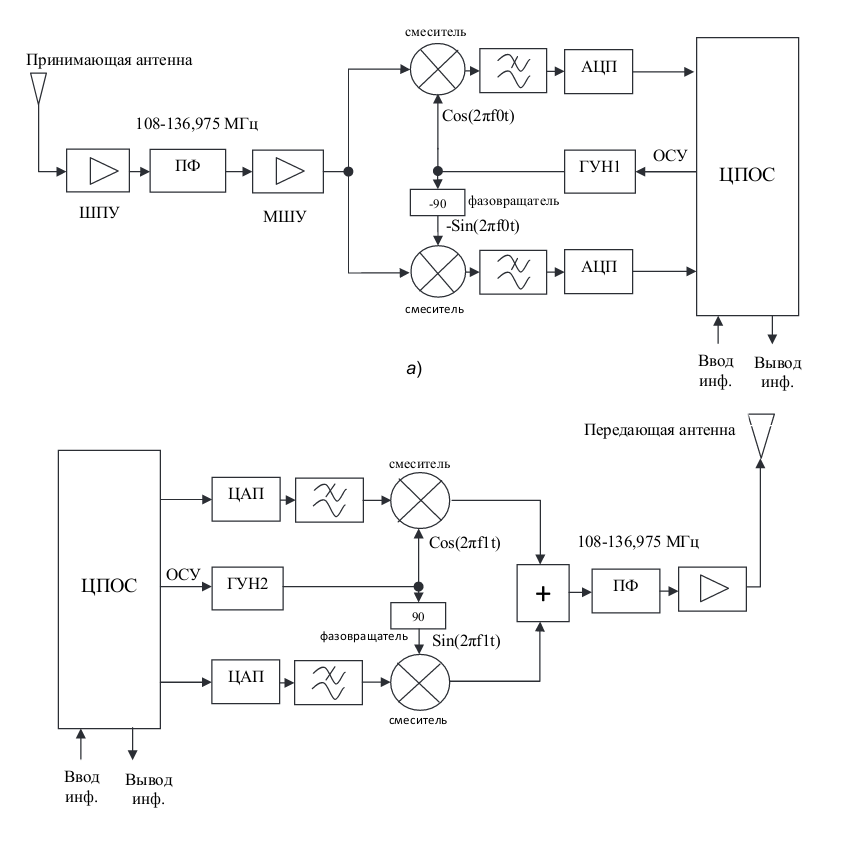
\includegraphics[width=0.9\textwidth]{vdl4}
  \caption{функциональная схема транспондера VDL-4}
\end{figure}

\begin{itemize}
\item [ЦПОС] Центральный процессор обработки сигналов
\item [МШУ] Малошумящий усилитель
\item [ГУН] Генератор управляемый напряжением
\item [ПФ] Полосовой фильтр
\item [АЦП] Аналогово-цифвровой преобразователь
\item [ЦАП] Цифро-аналоговый преобразователь
\end{itemize}
\newpage

\section{Система индикации}
Система индикации будет получать данные от транспондера в виде сформированного
текстового файла, возможна реализация тестового режима в котором будут показаные
тестовые (не соотвествующие действительности) объекты сети, с целью проверки
работоспособности системы индикации как таковой.

\subsection{Основные требования}
Система индикации должна:
\begin{itemize}
\item Показывать текущее положение объекта на котором установлена данная система
  (себя)
\item Показывать радиус действия прямого радиодоступа - 400км
\item Показывать другие объекты сети:
  \begin{itemize}
  \item Самолеты, находящиеся в радиусе прямого радиодоступа
  \item Самолеты, находящиеся в зоне действия сети (при запросе расширения зоны
    наблюдения)
  \item Наземные и водные станции
  \end{itemize}
\item Планируемый курс определенного объекта (по запросу)
\end{itemize}

Для тестового режима, реализуемого в данной работе реализуем следующий
функционал:
\begin{itemize}
\item Показываем себя - самолет летящий с фиксированным курсом и скоростью из
  начальных координат г. Москвы.
\item 2-3 самолета, летящих недалеко от нас с фиксированными курсами и
  скоростями.
\item Самолеты, покинувшие область прямого радиодоступа будут помечаться как
  самолеты ``в сети'' пока расстояние до них не станет больше 800км, после чего
  они полностью исчезнут с карты, до тех пор пока мы не встретимся с ними снова.
\end{itemize}

\subsection{Тенические требования}
Система индикации должна работать на основных платформах: Microsoft\copyright
Windows\copyright, Mac OS X, Linux с системой окон X11. Так же желательна
поддержка мобильных систем Android и Apple iOS.
\newpage

\chapter{Разработка прикладного алгоритмического и  програмного
  обеспения  системы индикации} %8 pages 
\section{Выбор платформы}
Для поддержания наибольшего числа платформ и легкости разработки, поддержки и
разработки системы индикации, я решил использовать платформу HTML5. Система
индикации (в дальшейшем СИ) написана на языке JavaScript с использованием
нескольких сторонних библиотек.

\subsection{Особенности платформы}
СИ может быть запущена из практически любого современного браузера - IE11,
Firefox, Chrome, Safari, но в целях удобства и потенциальной возможности доступа
к аппаратной части я использовал оболочку Electron - окружение позволяющее
написать приложение целиком на JavaScript\\HTML5 и при этом иметь функционал
``родного'' приложения - доступ к файловой системе, внешним устройствам,
функционалу конкретной операционной системе (уведомления, интеграция).

\subsection{Используемые технологии}
СИ в большей части использует библиотеку обработки и отображения данных - d3.js.
Данная библиотека позволяет, на основании входных данных выполнять определенные
действия - создавать, изменять, удалять указанные узлы. В данной работе при
помощи этой библиотеки управляется SVG элементы, строящие векторное
представление ортографической проекции земного шара (границы суши и земли) и
объектов нахоящихся на нём. Библиотека так же позволяет напрямую использовать
координаты в формате широта-долгота.

\subsection{Алгоритим программы}
Алгоритм программы заключается в следующем:
\begin{itemize}
\item Получить данные от транспондера (или сформировать их для тестового режима)
\item Нормализовать данные, обновить внутренний образ сети на их основе (в
  тестовом режиме данные обновляются за счет предыдущего состояния)
\item Передать данные о координатах в объекты d3.js
\item Модифицировать объекты d3.js для отображения дополнительной информации
  (направление, бортовой номер, скорость, тип)
\item Повторить все шаги снова по прохождении интервала обновления
\end{itemize}
\newpage

Исходный код программы:

\lstinputlisting[caption=client/index.js]{../client/index.js}
\lstinputlisting[caption=app.js]{../app.js}
\lstinputlisting[caption=index.html]{../index.html}

\newpage
\chapter{Разработка инструкции по эксплуатации}
\newpage
\chapter{Разработка вопросов по экологии и безопасности жизнидеятельности при
  работе с электронной аппаратурой (ЭА)} %8 pages
\section{Эргономические требования к рабочему месту при работе с ЭА}
Основные требования к рабочему месту оператора наземной станции:

\begin{itemize}
\item правильное размещение рабочего места в производственном помещении; 
\item выбор эргономично обоснованного рабочего положения, производственных
  мебели с учетом антропометрическими характеристик человека; 
\item рациональное расположение оборудования. 
\end{itemize}

Общие принципы организации рабочего места:

\begin{itemize}
\item на рабочем месте не должно быть ничего лишнего. Все Необходимые для работы
  предметы должны быть рядом с работником, но не мешать ему; 
\item то предметы, которыми пользуются чаще, располагаются ближе, чем предметы,
  которыми пользуются реже; 
\item если используют обе руки, то местоположение приспособлений выбирается с
  учетом удобства захвата его двумя руками; 
\item рабочее место не должно быть загромождено; 
\item организация рабочего места должна обеспечивать необходимую обзорность 
\end{itemize}

Статические напряжения работника в процессе труда связаны с поддержания в
неподвижно состоянии предметов и орудий труда, а также поддержание рабочей позы 
% нормы
\section{Микроклиматические условия в производственном помещении  при работе с ЭА}
% температура, влажность, нормы
Нормы производственного микроклимата установлены в СанПиН 2.2.4.548-96
«Гигиенические требования к микроклимату производственных помещений» 

Они едины для всех производств и всех климатических зон с некоторыми
незначительными отступлениями. 

В этих нормах отдельно нормируется каждый компонент микроклимата в рабочей зоне
производственного помещения: температура, относительная влажность, скорость
движения воздуха в зависимости от способности организма человека к
акклиматизации в разное время года, характера одежды, интенсивности производимой
работы и характера тепловыделений в рабочем помещении. 

Работа оператора наземной станции подходит под категорию Iа -- работы с
интенсивностью энерготрат до 120 ккал/ч (до 139 Вт), производимые сидя и
сопровождающиеся незначительным физическим напряжением (ряд профессий на 
предприятиях точного приборо- и машиностроения, на часовом, швейном
производствах, в сфере управления и т.п.). 

\hyphenpenalty 100000
\begin{table}[!h]
  \caption{Требования по микроклимату к категории Iа}
  \begin{tabular}{|l|p{2.75cm}|p{2.75cm}|p{2.75cm}|p{2.75cm}|}
    \hline
    Период года & Темп. воздуха, C\degree & Темп. поверхностей, C\degree & Отн. влажность воздуха, \% & Скорость движения воздуха, \%\\
    \hline
    Холодный    & 22---24               & 21---25                    & 60---40                           & 0.1                       \\
    \hline
    Теплый      & 23---25               & 22---26                    & 60---40                           & 0.1                     \\
    \hline
  \end{tabular}
\end{table}
\exhyphenpenalty 10000

\section{Освещенность в производственном помещении при работе  с ЭА}

Расчитаем необоходимое количество осветительных приборов в произодственном
помещении -- комнате операторов наземной станции. В соответсвии с нормами СанПиН
2.2.2/2.4.1340-03 освещенность на поверхности стола должна быть 300--500лк,
возьмем среднее -- $E_{min} = 400лк$.

Необходимое количество приборов высчитывается по формуле:
\[
N = \frac{ E_{min} \cdot S \cdot k }{ F_{\Lambda} \cdot z \cdot n \cdot \eta }
\]

где \\
$S$ -- площадь пола в помещении \\
$k$ -- коэфициент запаса \\
$F_{\Lambda}$ -- световой поток, создаваемый одной лампой. В нашем случае
используем лампы ИКЕЯ ЛЕДАРЕ с заявленным световым потоком $400$ лм \\
$n$ -- количество ламп в светильнике -- в нашем случае -- $1$ \\
$\eta$ -- коэфициент использования светового потока, зависит от показателя
помещения $\varphi$, коэфициентов отражения  ($\rho_{\text{стен}}$) и потолка
($\rho_{\text{пот}}$) и расчитывается из таблицы\\
$z$ -- коэфициент неравномерности освещенности, пример равным $0.8$

Показатель помещения $\varphi$ расчитывается по формуле:
\[
\varphi = \frac{A \cdot B}{H_{P} \cdot (A + B)}
\]

Где $A$ и $B$ -- ширина и длина помещения, м; $H_{P}$ -- высота подвеса
светильника, расстояние между рабочей поверхностью и светильником. В нашем
случае возьмем $A = B = 3\text{м}$ а $H_{P} = 1.4\text{м}$. Показатель помещения
будет равен 
\[
\varphi = \frac{3^2}{1.4*(3*2)} = \frac{9}{1.4*6} = \frac{9}{8.4} = 1.07
\]
По таблице
\footnote{\url{http://www.malahit-irk.ru/index.php/2011-01-13-09-04-43/202-2011-07-07-12-57-50.html}} 
найдем значение $\eta$ приняв коэфициенты отражения пола и потолка 70\% и 50\%
соответственно.

$\eta = 49$

коэфициент запаса для светодиодных ламп - $k = 11$
\footnote{\url{http://www.axiomasveta.com/info/koeffitsient_zapasa/}} 

Расчитаем необходимое количество осветительных приборов:
\[
N = \frac{ 400 \cdot 9 \cdot 1.1 }{ 400 \cdot 0.8 \cdot 1 \cdot 49 } = 0.25
\]

Для такого помещения достаточно одной ламы.
\section{Режим труда и отдыха при работе с ЭА}

Согласно СанПиН 3.3.2.007-98 в течение дня должны предусматриваться:

\begin{itemize}
\item перерывы для отдыха и употребления пищи (обеденные перерывы);
\item перерывы для отдыха и личных нужд (согласно трудовым нормам);
\item дополнительные перерывы, которые вводятся для отдельных профессий с учетом особенностей трудовой деятельности.
\end{itemize}

При работе оператор наземной станции должен выходить на перерыв минимум три
раза, из которых 30 мин обеденный перерыв и 30 минут на личные нужды и отдых.

\section{Вывод}
В данной работе мною были рассмотрены основные вопросы безопасности
жизнедеятельности и охраны труда оператора наземной станции наблюдения. Для того
чтобы поддерживать охрану труда на рабочем месте нужно придерживаться расчитаных
и выписанных мною норм. %насрать. я ебал. пизда.
\newpage
\chapter{Технико-экономическеой обоснование. Сравнение системы индиации с
  аналогами с помощью метода анализа иерархий} %8 pages
\section{Постановка задачи}
Цель расчетов в данной задаче - сравнить использование данной системы индикации
с аналогами используя метод анализа иерархий (МАИ).
% TODO описать аналоги.

\begin{table}[!h]
  \caption{Исходные данные, аналоги системы индикации}
  \begin{tabular}{ | r | p{6cm} | l | l |}
    \hline
    Показатель   & СИ рассм. в данной работе                  & ADS-B View    & Avare  \\
    \hline
    Платформы    & Win, Mac, Linux, FreeBSD, Android, iOS, WP & iOS           & Android \\
    \hline
    Лицензия ПО  & GPLv3                                      & Проприетарная & Apache 2.0 \\
    \hline
    Поддержка    & Авторская (по возможности)                 & Коммерческая  & Cообщество \\
    \hline
  \end{tabular}
\end{table}

\section{Иерархическое представление задачи}
На верхнем иерархическом уровне основная задача - выбрать наилучший вариант
системы индикации, в сравнении с нескольими аналогами. На промежуточных уровнях
- выбор альтернатив по системе критериев.

Нам необходимо определиться с важностью критериев при выборе наилучшего
варианта. Приоритет определяется путем попарного сравнения критериев.
\subsection{Сравнение критериев}
Сравним в деталях каждый показатель (критерий) с каждым.
\subsubsection{Платформы vs. Лицензия}
Количество поддерживаемых платформ дает больший выбор используемого ``железа''
для системы, не обязательно покупать оборудование конкретного производителя
из-за того что ПО этого требует.

С другой стороны открытая лицензия позволяет (как правило) иметь доступ к
исходному коду ПО и возможность его изменять - это дает возможность
самостоятельно исправить неполадку не дожидаясь официальной тех.поддержки и
бюрократии, однако в целом принято считать что коммерческие продукты обладают
лучшим качеством в сравнении с открытыми.

\textbf{Итого:} 2 к 1 в пользу платформ
\subsubsection{Лицензия vs. Поддержкa}
Критерий лицензии обсуждался выше. Техническая поддержка ПО зачастую имеет
решающую роль при выборе программного решения. В нашем случае, кажется что
лицензия и поддержка равносильны и взаимоисключаемы - либо есть исходный код и
его можно править, либо есть техподдержка которая исправит любую неполадку. Оба
случая видятся равноценными по затратам.

\textbf{Итого:} 1 к 1
\subsubsection{Платформы vs. Поддержка}
Помимо сказанного выше стоит добавить пару слов конкретно к этому сравнению. ПО
написанное под несколько платформ сразу зачастую пишется на ЯП с низким порогом
вхождения (Java, JavaScript), что облегчает поддержку ПО собственными
средствами.

Так же хочется сказать что при неисправности платформы, если ПО зависит от неё
придется общаться с техподдержкой платформы, в то время как платформонезависимое
ПО можно просто установить на другой платформе.

\textbf{Итого:} 2 к 1 в пользу платформ
\subsubsection{Заключение}
Построим матрицу сравнений
\begin{table}[h]
  \caption{матрица сравнений}
  \begin{tabular}{l|c|c|c|}
    \cline{2-4}
    {}                              & \multicolumn{1}{l|}{Платформы} & \multicolumn{1}{l|}{Лицензия} & \multicolumn{1}{l|}{Поддержка} \\ \hline
    \multicolumn{1}{|l|}{Платформы} & 1                              & 2                             & 2                              \\ \hline
    \multicolumn{1}{|l|}{Лицензия}  & $0.5$                          & 1                             & 1                              \\ \hline
    \multicolumn{1}{|l|}{Поддержка} & $0.5$                          & 1                             & 1                              \\ \hline
  \end{tabular}
\end{table}

\subsection{Сравнение альтернатив}
Аналогично сравним альтернативы по критериям

\begin{table}[h]
  \caption{матрица сравнений по платформам}
  \begin{tabular}{l|c|c|c|}
    \cline{2-4}
    {}                               & \multicolumn{1}{l|}{СИ}        & \multicolumn{1}{l|}{ADS-B View} & \multicolumn{1}{l|}{Avare} \\ \hline
    \multicolumn{1}{|l|}{СИ}         & 1                              & 8                               & 6                          \\ \hline
    \multicolumn{1}{|l|}{ADS-B View} & 0.125                          & 1                               & 0.5                        \\ \hline
    \multicolumn{1}{|l|}{Avare}      & 0.165                          & 2                               & 1                          \\ \hline
  \end{tabular}
\end{table}

\begin{table}
  \caption{матрица сравнений по лицензиям}
  \begin{tabular}{l|c|c|c|}
    \cline{2-4}
    {}                               & \multicolumn{1}{l|}{СИ}        & \multicolumn{1}{l|}{ADS-B View} & \multicolumn{1}{l|}{Avare} \\ \hline
    \multicolumn{1}{|l|}{СИ}         & 1                              & 3                               & 1                          \\ \hline
    \multicolumn{1}{|l|}{ADS-B View} & 0.333                          & 1                               & 0.333                      \\ \hline
    \multicolumn{1}{|l|}{Avare}      & 1                              & 3                               & 1                          \\ \hline
  \end{tabular}
\end{table}

\begin{table}
  \caption{матрица сравнений по поддерке}
  \begin{tabular}{l|c|c|c|}
    \cline{2-4}
    {}                               & \multicolumn{1}{l|}{СИ}        & \multicolumn{1}{l|}{ADS-B View} & \multicolumn{1}{l|}{Avare} \\ \hline
    \multicolumn{1}{|l|}{СИ}         & 1                              & 0.165                           & 0.25                       \\ \hline
    \multicolumn{1}{|l|}{ADS-B View} & 6                              & 1                               & 2                          \\ \hline
    \multicolumn{1}{|l|}{Avare}      & 4                              & 0.5                             & 1                          \\ \hline
  \end{tabular}
\end{table}
\subsection{Синтез приоритетов}
Вычислим вектора приоритетов для критериев и альтернатив

\subsubsection{Критерии}
% Описать что мы тут бля делаем
$ b_1=\sqrt[3]{1 \cdot 2 \cdot 2} = \sqrt[3]{2} = 1.2599210499 $ \\
$ b_2=\sqrt[3]{0.5 \cdot 1 \cdot 1} = \sqrt[3]{0.5} = 0.793700525984 $ \\
$ b_3=\sqrt[3]{0.5 \cdot 1 \cdot 1} = \sqrt[3]{0.5} = 0.793700525984 $ \\
\\
$ S = 1.2599210499 + 0.793700525984 + 0.793700525984 = 2.84732210 $ \\
\\
$K_1 = b_1/S = 0.44249333 $ \\
$K_2 = b_2/S = 0.35120719 $ \\
$K_3 = b_3/S = 0.35120719 $ \\

\subsubsection{Платформы}
$ b_1=\sqrt[3]{1 \cdot 8 \cdot 6} = \sqrt[3]{48} = 3.63424118566 $ \\
$ b_2=\sqrt[3]{0.125 \cdot 1 \cdot 0.5} = \sqrt[3]{0.0625} = 0.396850262992 $ \\
$ b_3=\sqrt[3]{0.165 \cdot 2 \cdot 1} = \sqrt[3]{0.33} = 0.691042323001 $ \\
\\
$ S = 3.63424118566 + 0.396850262992 + 0.691042323001 = 4.72213377 $ \\
\\
$ X_1 = b_1/S = 0.76961843 $ \\
$ X_2 = b_2/S = 0.08404045 $ \\
$ X_3 = b_3/S = 0.14634112 $ \\

\subsubsection{Лицензия}
$ b_1=\sqrt[3]{1 \cdot 3 \cdot 1} = \sqrt[3]{3} = 1.44224957031 $ \\
$ b_2=\sqrt[3]{0.333 \cdot 1 \cdot 0.333} = \sqrt[3]{0.110889} = 0.480429303424
$ \\
$ b_3=\sqrt[3]{1 \cdot 3 \cdot 1} = \sqrt[3]{3} = 1.44224957031 $ \\
\\
$ S = 1.44224957031 + 0.480429303424 + 1.44224957031 = 3.36492844 $ \\
\\
$ Y_1 = b_1/S = 0.42861226 $ \\
$ Y_2 = b_2/S = 0.14277549 $ \\
$ Y_3 = b_3/S = 0.42861226 $ \\

\subsubsection{Поддержка}
$ b_1=\sqrt[3]{1 \cdot 0.165 \cdot 0.25} = \sqrt[3]{0.04125} = 0.345521161501 $ \\
$ b_2=\sqrt[3]{6 \cdot 1 \cdot 2} = \sqrt[3]{12} = 2.28942848511 $ \\
$ b_3=\sqrt[3]{4 \cdot 0.5 \cdot 1} = \sqrt[3]{2} = 1.2599210499 $ \\
\\
$ S = 0.345521161501 + 2.28942848511 + 1.2599210499 = 3.89487070 $ \\
\\
$ Z_1 = b_1/S = 0.08871184 $ \\
$ Z_2 = b_2/S = 0.58780603 $ \\
$ Z_3 = b_3/S = 0.32348212 $ \\

\subsection{Расчет глобальных приоритетов}
Расчет глобальных приоритетов производится по функции: \\
$P_i=X_i \cdot K_1 + Y_i \cdot K_2 + Z_i \cdot K_3 $ \\
\\
$P_{СИ} = 0.44249333 * 0.76961843 + 0.35120719 * 0.42861226 + 0.35120719 *
0.08871184 = 0.52223897$ \\
$P_{ADS-B View} = 0.44249333 * 0.08404045 + 0.35120719 * 0.14277549 + 0.35120719
* 0.58780603 = 0.29377282 $ \\
$P_{Avare} = 0.44249333 * 0.14634112 + 0.35120719 * 0.42861226 + 0.35120719 *
0.32348212 = 0.32889592$ \\
\\
Из вычислений видно что наилучший выбор - СИ реализуемая в данной работе.
Наилушчий по большему счету из-за количества поддерживаемых платформ. На втором
месте стоит Avare, за счет открытости и поддержке платформы Android, на которой
работает большое число взаимозаменяемого оборудования.

\newpage
\chapter{Заключение}
\end{document}